\documentclass{article}
\usepackage{graphicx} % Required for inserting images
\usepackage{amsmath}
\usepackage{hyperref}
\usepackage{subcaption}
\usepackage{tikz}
\usepackage{listings}
\usepackage{xcolor}

\definecolor{codegreen}{rgb}{0,0.6,0}
\definecolor{codegray}{rgb}{0.5,0.5,0.5}
\definecolor{codepurple}{rgb}{0.58,0,0.82}
\definecolor{backcolour}{rgb}{0.95,0.95,0.92}

\lstdefinestyle{mystyle}{
    backgroundcolor=\color{backcolour},   
    commentstyle=\color{codegreen},
    keywordstyle=\color{magenta},
    numberstyle=\tiny\color{codegray},
    stringstyle=\color{codepurple},
    basicstyle=\ttfamily\footnotesize,
    breakatwhitespace=false,         
    breaklines=true,                 
    captionpos=b,                    
    keepspaces=true,                 
    numbers=left,                    
    numbersep=5pt,                  
    showspaces=false,                
    showstringspaces=false,
    showtabs=false,                  
    tabsize=2
}

\lstset{style=mystyle}

\usetikzlibrary{shapes,arrows}

\newcommand{\Lp}[1]{\mathcal{L}\left[#1\right](s)}

\title{Automatique TP3}
\author{Atik Anis, Alexis Brossier}
\date{11 avril 2024}

\begin{document}
\begin{titlepage}
    \maketitle
\end{titlepage}

\section{Préparation}
\subsection{Fonction de transfert}
\begin{gather*}
    J\frac{d^2\theta}{dt^2}+D\frac{d\theta}{dt}+K_s\theta=\tau_\theta=K_tV\\
    \Leftrightarrow J\Lp{\frac{d^2\theta}{dt^2}}+D\Lp{\frac{d\theta}{dt}}+K_s\Lp{\theta}=K_t\Lp{V}\\
    \Leftrightarrow JY(s)s^2+DY(s)s+K_sY(s)=K_tU(s)\\
    \Leftrightarrow Y(s)=\frac{K_tU(s)}{Js^2+Ds+K_s}\\
    H(s)=\frac{Y(s)}{U(s)}=\frac{K_t}{Js^2+Ds+K_s}=\frac{\frac{K_t}{K_s}}{\frac{J}{K_s}s^2+\frac{D}{K_s}s+1}\\
\end{gather*}
On peut identifier les coefficients suivants :
\begin{equation*}
    \begin{cases}
        K=\frac{K_t}{K_s}\\
        \frac{1}{\omega_n^2}=\frac{J}{K_s}\\
        \frac{2\zeta}{w_n}=\frac{D}{K_s}\\
    \end{cases}
    \Leftrightarrow
    \begin{cases}
        K=\frac{K_t}{K_s}\\
        \omega_n=\sqrt{\frac{K_s}{J}}\\
        \zeta=\frac{D\omega_n}{2K_s}=\frac{D\sqrt{\frac{K_s}{J}}}{2K_s}\\
    \end{cases}
\end{equation*}
\subsection{Correcteur PIV}
On a la commande d'entrée suivante :
\begin{align*}
    u(t)&=K_p\left[e(t)+\frac{1}{T_i}\int_0^te(\tau)d\tau\right]-K_d\frac{dy(t)}{dt}\\
    U(s)&=\Lp{u(t)}=K_p\Lp{e(t)}+\frac{K_p}{T_i}\Lp{\int_0^te(\tau)d\tau}-K_d\Lp{\frac{dy(t)}{dt}}\\
    &=K_pE(s)+\frac{K_p}{T_i}\frac{E(s)}{s}-K_dY(s)s=(1+\frac{1}{T_is})K_pE(s)-K_dsY(s)
\end{align*}
On peut alors identifier les correcteurs suivants
\begin{equation*}
    \begin{cases}
        C_{P1}(s)=K_p(1+\frac{1}{T_is})\\
        C_D(s)=K_ds
    \end{cases}
\end{equation*}
\subsection{Schéma Bloc-Diagramme}
\begin{figure}[h]
    \centering
    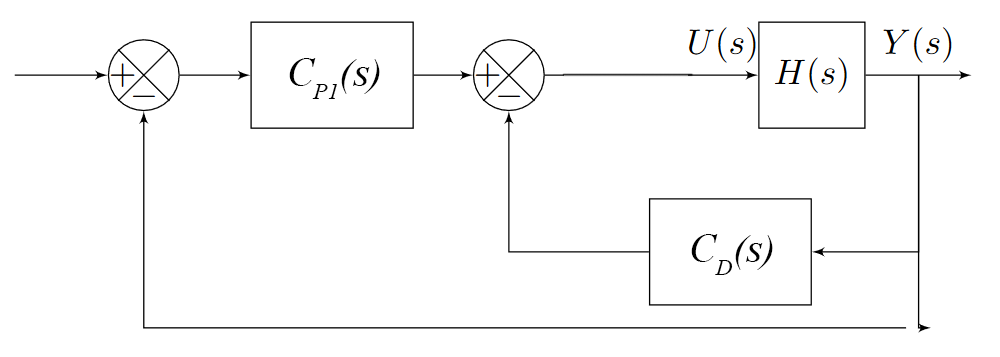
\includegraphics[width=\linewidth]{piv.png}
    \caption{Bloc Diagramme du correcteur PIV}
    \label{fig:diagram}
\end{figure}
\subsection{Fonction de transfert rétroactive}
D'après la règle de Mason :
\begin{align*}
    H_1(s)&=\frac{H(s)}{1+C_D(s)H(s)}=\frac{\frac{K}{\frac{s^2}{\omega_n^2}+\frac{2\zeta}{\omega_n}s+1}}{1+K_ds\frac{K}{\frac{s^2}{\omega_n^2}+\frac{2\zeta}{\omega_n}s+1}}\\
    &=\frac{K}{\frac{s^2}{\omega_n^2}+(\frac{2\zeta}{\omega_n}+K_dK)s+1}
\end{align*}
On peut alors identifier les coefficients selon une forme canonique du second degré :
\begin{equation*}
    \begin{cases}
        K_1=K\\
        \frac{1}{\omega_1^2}=\frac{1}{\omega_n^2}\\
        \frac{2\zeta_1}{\omega_1}=\frac{2\zeta}{\omega_n}+K_dK\\
    \end{cases}
    \Leftrightarrow
    \begin{cases}
        K_1=K\\
        \omega_1=\omega_n\\
        \zeta_1=\frac{\omega_n(\frac{2\zeta}{\omega_n}+K_dK)}{2}=\frac{2\zeta+K_dK\omega_n}{2}\\
    \end{cases}
\end{equation*}
\section{Analyse du système en boucle ouverte}
\subsection{Diagramme de Bode en boucle ouverte}
\begin{figure}[h]
    \centering
    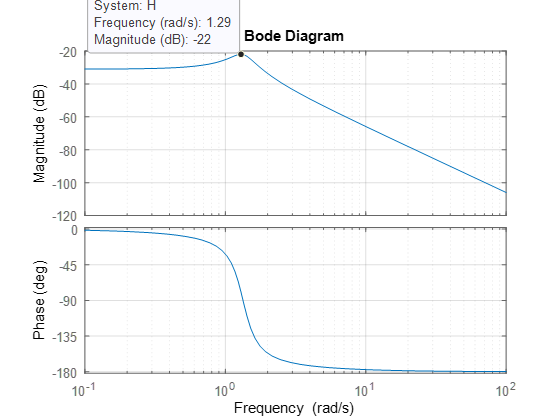
\includegraphics[width=\linewidth]{bode313.png}
    \caption{Diagramme de Bode en boucle ouverte}
    \label{fig:bode313}
\end{figure}
On remarque sur la figure \ref{fig:bode313} que pour les petites fréquences $\omega\rightarrow0$, le système se comporte en système proportionnel confirmé par la pente de 0dB/décade. En revanche, pour les hautes fréquences $\omega\rightarrow+\infty$, le système se comporte en double intégrateur dû à la pente de -40dB/décade.
On peut également remarquer une résonance à $\omega\approx1.29$ rad/s. Cette résonance est liée au fait que la valeur de $\zeta=0.1794$ est au-dessous de 0.7 ($\approx\frac{\sqrt{2}}{2}$).
\subsection{Réponse indicielle en boucle ouverte}
On obtient un temps de réponse de 12.3 secondes, un temps de montée de 0.894s, un dépassement de 56\% et une période d'oscillation de 4.78 secondes. cf. figure \ref{fig:step314}.

\begin{figure}[h]
    \centering
    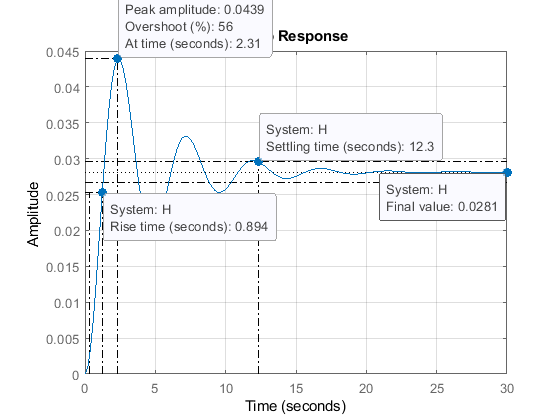
\includegraphics[width=1\linewidth]{step314.png}
    \caption{Réponse indicielle du système en boucle ouverte}
    \label{fig:step314}
\end{figure}

La réponse indicielle est la réponse du système face à l'échelon comme valeur d'entrée. Le dépassement est plutôt élevé, le but du correcteur va donc être de diminuer ce dépassement et de diminuer le temps de réponse et de globalement atténuer les oscillations. On peut également noter que la valeur finale correspond à la valeur de K ($\approx 0.028$).
\section{Synthèse de correcteur PIV}
\subsection{Calcul de $K_d$}
On souhaite trouver la valeur de $K_d$ tel que :
\begin{align*}
    \zeta_1&=\frac{2\zeta+K_dK\omega_n}{2}=0.7\\
    \Leftrightarrow K_d&=\frac{2(\zeta_1-\zeta)}{K\omega_n}\approx27.7
\end{align*}
\subsection{Réponse indicielle}
On compare sur la figure \ref{fig:step323} les réponses indicielles de H(s) (système en boucle ouverte sans correcteur) et $H_1(s)$ (système en boucle fermée avec correcteur dérivateur $C_D(s)$). On remarque que la réponse indicielle de $H_1$ présente bien moins de perturbations que H, ce qui mène à un temps de réponse bien diminué (1.59 seconde pour $H_1$ contre 12.3 secondes pour H). Le système en boucle fermée présente aussi un dépassement moindre par rapport à H, en effet le dépassement maximal est de 4.6\% contre 56\% pour H. Cependant on remarque que le temps de montée a légèrement augmenté et est passé de 0.894 seconde à 1.69 seconde. La valeur finale reste inchangée entre H et $H_1$. Notre correcteur $C_D$ a introduit une force mécanique similaire au frottement visqueux permettant d'amortir la réponse du système (car on a fixé $\zeta_1 = 0.7$).
\begin{figure}[h]
    \centering
    \begin{subfigure}{\textwidth}
        \centering
        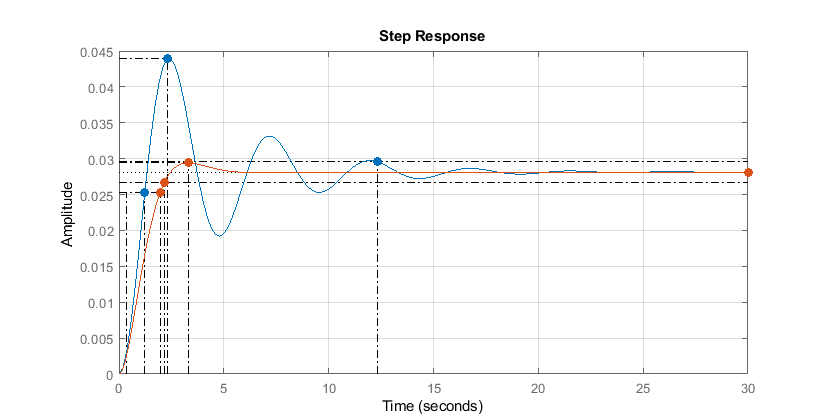
\includegraphics[width=\textwidth]{step323.png}
    \end{subfigure}
    \hfill
    \begin{subfigure}{\textwidth}
        \centering
        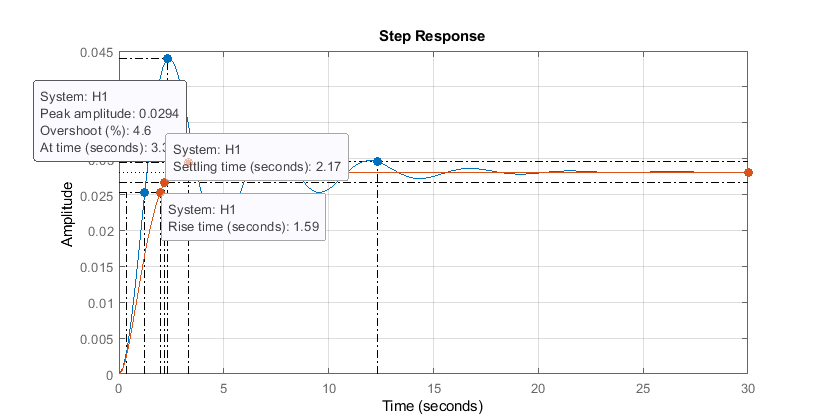
\includegraphics[width=\textwidth]{step323_d.png}
    \end{subfigure}
    \caption{Réponses indicielles de H (courbe bleue) et $H_1$ (courbe orange)}
    \label{fig:step323}
\end{figure}
\subsection{Diagramme de bode de $H_0$ et marge de phase}
\begin{figure}[h]
    \centering
    \begin{subfigure}{0.45\textwidth}
        \centering
        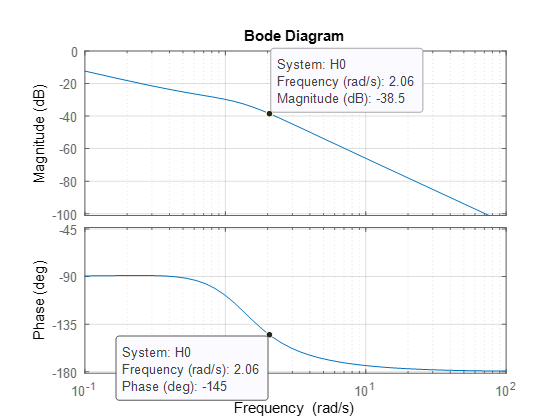
\includegraphics[width=1\textwidth]{bode325.png}
        \label{fig:bode325}
    \end{subfigure}
    \hfill
    \begin{subfigure}{0.45\textwidth}
        \centering
        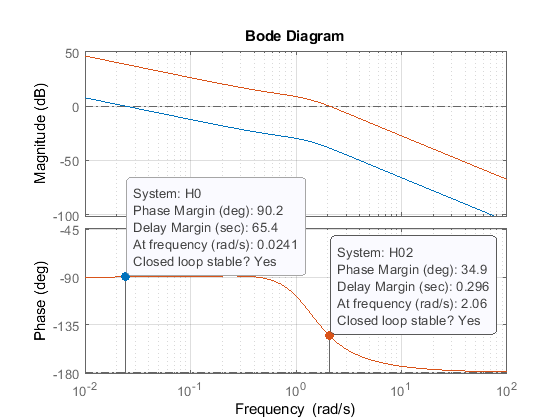
\includegraphics[width=1\textwidth]{bode325_2.png}
        \label{fig:bode325_2}
    \end{subfigure}
    \caption{Diagramme de bode de $H_0$ pour $K_p=1$ et $K_p=84.14$}
\end{figure}
On remarque que pour atteindre une marche de phase a 35°, on doit monter le gain de +38.5 dB (cf. figure \ref{fig:bode325}), soit :
\begin{gather*}
    20\log(K_p)=38.5\\
    K_p=10^{\frac{38.5}{20}}\\
    K_p=84.14
\end{gather*}
On prendra alors pour la suite une valeur de $K_p=84.14$.
En retraçant le diagramme de Bode pour cette valeur, on peut vérifier que la marge de phase a été décalé et est désormais à 35° comme souhaité.
\subsection{Réponse indicielle en boucle fermée}
On trace la réponse indicielle (cf. figure \ref{fig:step326}) en boucle fermée avec nos correcteurs $C_PI$ et $C_D$ comme indiqué dans le diagramme figure \ref{fig:diagram}.
On remarque un temps de montée qui est redescendu, mais au prix du retour de perturbations assez fortes (27.6\% avec les deux correcteurs contre 4.6\% avec seulement $C_D$ et 56\% sans correcteurs). Le retour des perturbations a également retardé le temps de réponse.
On remarque cependant que la valeur finale est égale à 1, ce qui correspond à notre signal d'entrée signifiant que notre système global à un gain unitaire.
\begin{figure}[h]
    \centering
    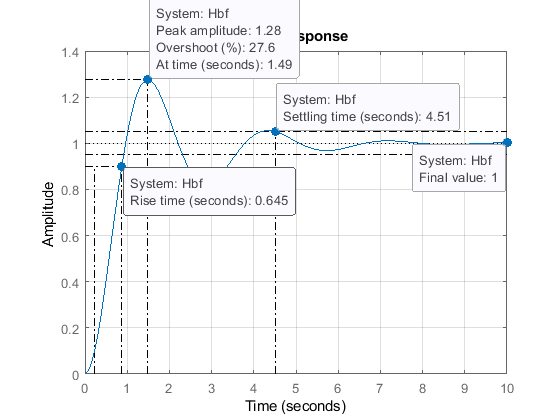
\includegraphics[width=1\linewidth]{step326.png}
    \caption{Réponse indicielle en boucle fermée avec les correcteurs}
    \label{fig:step326}
\end{figure}
\subsection{Conclusion}
On a étudié dans ce TP l'application d'un correcteur PIV dans le cadre d'un système électromécanique à 2 ddl. On a tout d'abord étudié le système sans correcteurs et on a pu remarquer que le système présentait de fortes perturbations et un temps de réponse très long. On a ensuite introduit le correcteur dérivateur qui a permis d'améliorer la stabilité du système et d'améliorer fortement le temps de réponse, cependant la précision du système restait mauvaise. On a enfin introduit le correcteur proportionnel-intégrateur qui a baissé légèrement la stabilité, mais a permis d'améliorer la précision de notre système, comme l'a montré une valeur de gain unitaire.

\clearpage
\section{Annexe}
Les fichiers (code source, fichier tex et images) sont également disponibles sur \href{https://github.com/AL3X-69/GEP2014L/blob/master/tp3.m}{GitHub}
\subsection{Code MATLAB}
\begin{lstlisting}
% GEP2014L Automatique
% Commande Servo

close all;

%% Analyse en boucle ouverte
J = 0.0219;
D = 0.0105;
Ks = 0.0391;
Kt = 0.0011;
s=tf('s');

K = Kt/Ks;
wn = sqrt(Ks/J);
z = D*wn/(2*Ks);

H=K/((s^2)/(wn^2) + 2*z*s/wn + 1);

% Diagramme de Bode en boucle ouverte
figure(1);
bode(H);

figure(2);
step(H);

%% Correcteur PIV
z1 = 0.7;
Kd = 2 * (z1 - z) / (K*wn);
Cd = Kd * s;
H1 = feedback(H, Cd);

figure(2);
hold on;
step(H1);
grid on;

figure(1);
hold on;
bode(H1);
grid on;

Ti = 1.17;
Kp = 1;
CPI = Kp * (1 + 1 / (Ti * s));
H0 = CPI * H1;
figure(3);
bode(H0);

Kp2 = 84.14;
CPI2 = Kp2 * (1 + 1 / (Ti * s));
H02 = CPI2 * H1;
figure(3);
hold on;
bode(H02);
grid;

Hbf = feedback(H02, 1);
figure(4);
step(Hbf);
grid;
\end{lstlisting}
\end{document}